% PLANTILLA APA7
% Creado por: Isaac Palma Medina
% Última actualización: 25/07/2021
% @COPYLEFT

% Fuentes consultadas (todos los derechos reservados):  
% Normas APA. (2019). Guía Normas APA. https://normas-apa.org/wp-content/uploads/Guia-Normas-APA-7ma-edicion.pdf
% Tecnológico de Costa Rica [Richmond]. (2020, 16 abril). LaTeX desde cero con Overleaf (1 de 3) [Vídeo]. YouTube. https://www.youtube.com/watch?v=kM1KvHVuaTY Weiss, D. (2021). 
% Formatting documents in APA style (7th Edition) with the apa7 LATEX class. https://ctan.math.washington.edu/tex-archive/macros/latex/contrib/apa7/apa7.pdf @COPYLEFT

%+-+-+-+-++-+-+-+-+-+-+-+-+-++-+-+-+-+-+-+-+-+-+-+-+-+-+-+-+-+-++-+-+-+-+-+-+-+-+-+

% Preámbulo
\documentclass[stu, 12pt, letterpaper, donotrepeattitle, floatsintext, natbib, helv]{apa7}
\usepackage[utf8]{inputenc}
\usepackage{comment}
\usepackage{marvosym}
\usepackage{graphicx}
\usepackage{float}
\usepackage[normalem]{ulem}
\usepackage[spanish]{babel} 
\usepackage{gensymb}
%\usepackage{titling}
\let\apasubparagraph\subparagraph
\let\subparagraph\paragraph
\usepackage[compact]{titlesec}
\let\subparagraph\apasubparagraph
\usepackage{hyperref}
\selectlanguage{spanish}
\useunder{\uline}{\ul}{}
\newcommand{\myparagraph}[1]{\paragraph{#1}\mbox{}\\}
\graphicspath{{./images/}}
\titleformat{\section}{\normalfont\large\bfseries}{\thetitle. \quad }{0pt}{}[{ \titlerule[0.8pt]}]
\titleformat{\subsection}{\normalfont\bfseries}{}{}{}[]

% Portada

\begin{document}
\begin{titlepage}
    \centering
    \vfill
    \LARGE Laboratorio \#8\\
    \vskip2cm
    \large Diego Quirós Artiñano \\
    Universidad Nacional de Costa Rica \\
    EIF-202: Soporte Técnico \\ 
    Carolina Gómez Fernández \\
    29 de mayo, 2022 \\
    \vfill
    
\includegraphics[width = 0.4\textwidth]{../../../UNAImage/UNA.png} \\
    \vfill
    \vfill
    % (autores separados, consultar al docente)
    % Manera oficial de colocar los autores:
    %\author{Autor(a) I, Autor(a) II, Autor(a) III, Autor(a) X}
\end{titlepage}

% Índices
\pagenumbering{roman}
    % Contenido
\addto\captionsspanish{
    \renewcommand*\contentsname{\largeÍndice}
}
\tableofcontents
\setcounter{tocdepth}{2}
\newpage
    % Figuras
\renewcommand{\listfigurename}{\largeÍndice de fíguras}
\listoffigures
\newpage
%     % Tablas
% \renewcommand{\listtablename}{\largeÍndice de tablas}
% \listoftables
% \newpage

% Cuerpo
\pagenumbering{arabic}

%------------------------------------------------------------------------------------
\section*{Introducción}
\phantomsection
\addcontentsline{toc}{section}{Introducción}

En este laboratorio se va a investigar sobre los USB booteables y los archivos .ISO que se usan para crearlos. Además de generar nuestros propios para practicar.

%------------------------------------------------------------------------------------
\section*{Hacer un Booteable USB}
\phantomsection
\addcontentsline{toc}{section}{Hacer un Booteable USB}

\begin{enumerate}
    \item Descargar el .ISO para crear el USB booteable. En mi caso para los dos ejemplos del laboratorio descargué:
    \begin{itemize}
        \item Manjaro porque me gusta esta versión de Arch Linux (https://manjaro.org/download/) (3.5GB)
        \item Windows 11 para ver como hacer la instalación de Windows (https://www.microsoft.com/software-download/windows11) (5.2GB)
    \end{itemize}
    \item Abra el software para flashear dirves. (Para esta instalación usé balenaEtcher)
    \item Seleccione el archivo .ISO que va a usar para la instalación
    \begin{figure}[H]
        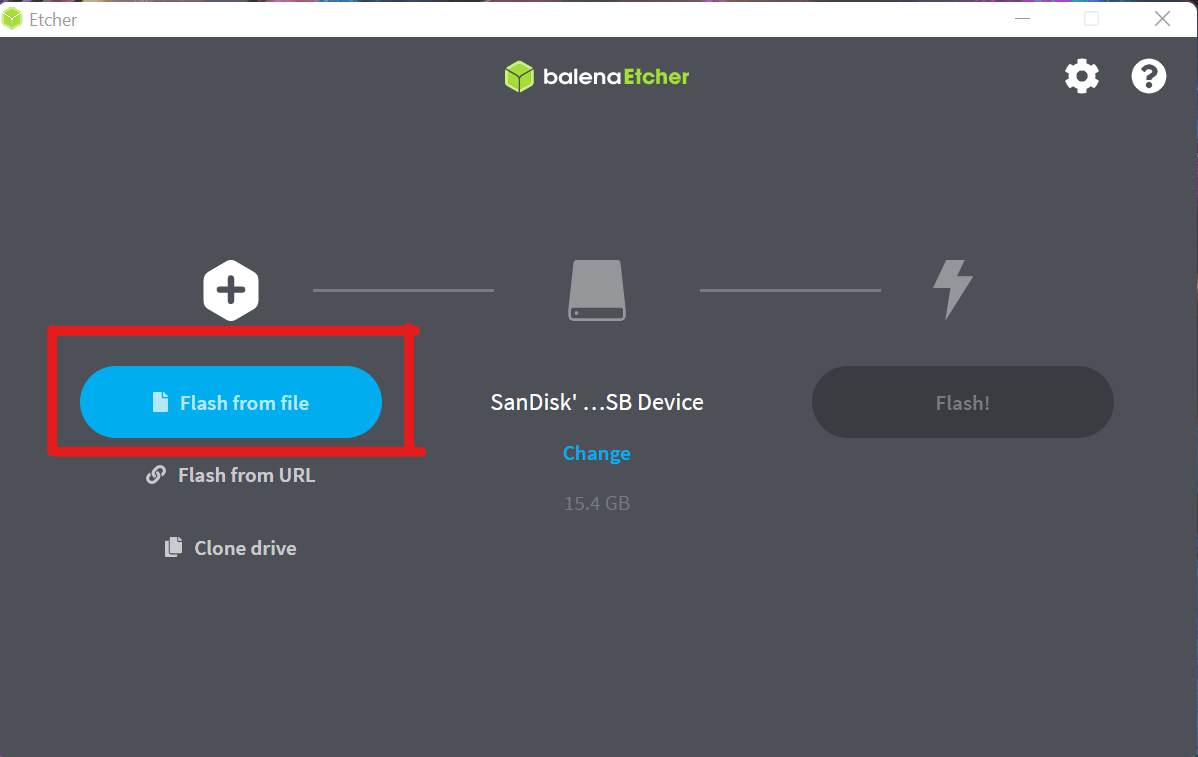
\includegraphics[width = 0.96\textwidth]{SelectISO.png}
        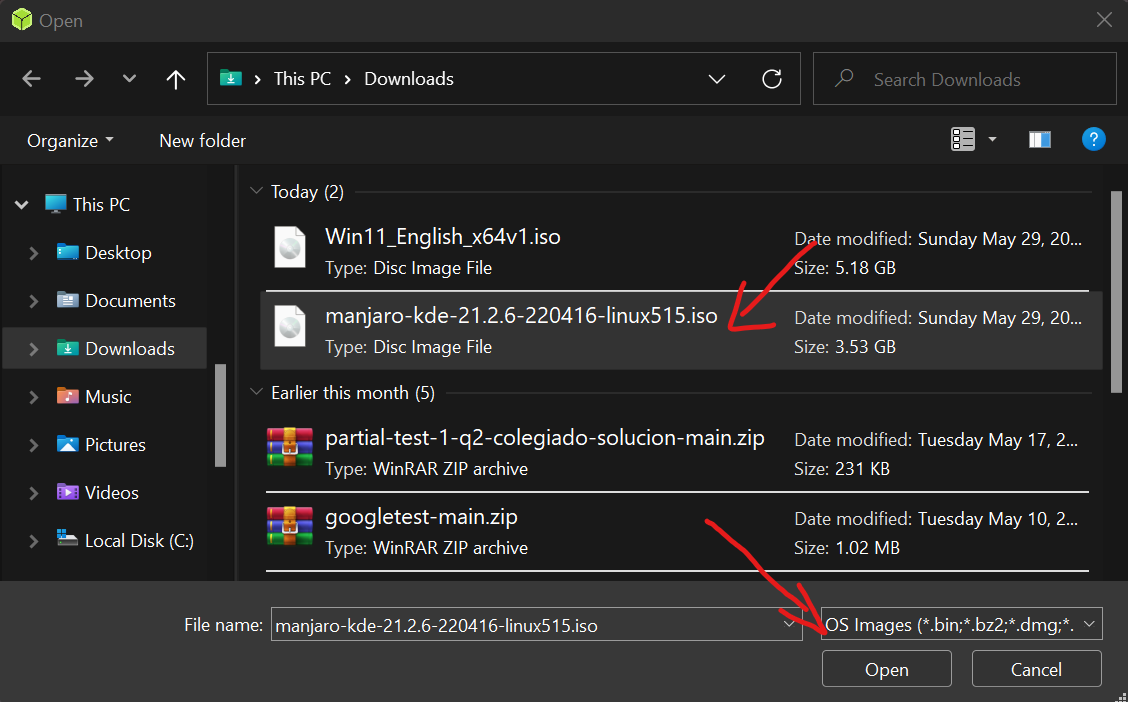
\includegraphics[width = 0.96\textwidth]{SelectISO2.png}
        \caption{Seleccionando el .ISO}
        \label{fig:selectingISO}
    \end{figure}
    \item Seleccione el USB que va a utilizar para hacer el live boot
    \begin{figure}[H]
        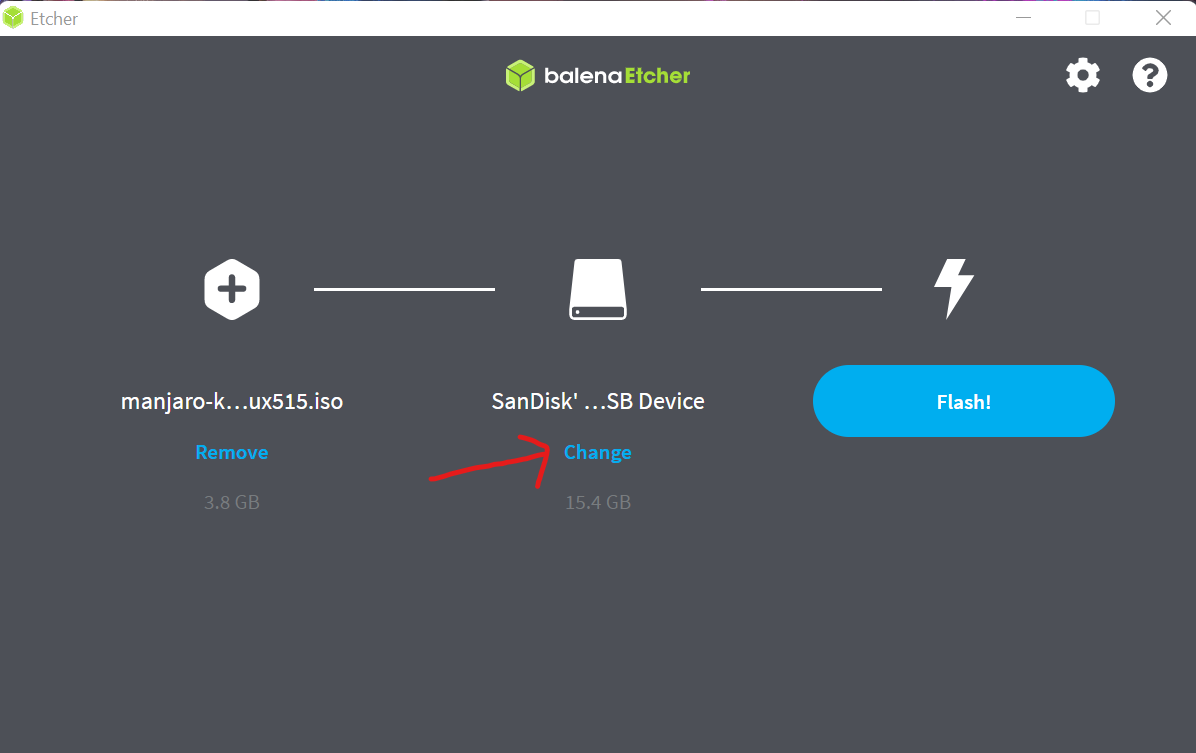
\includegraphics[width = 0.96\textwidth]{SelectUSBDevice.png}
        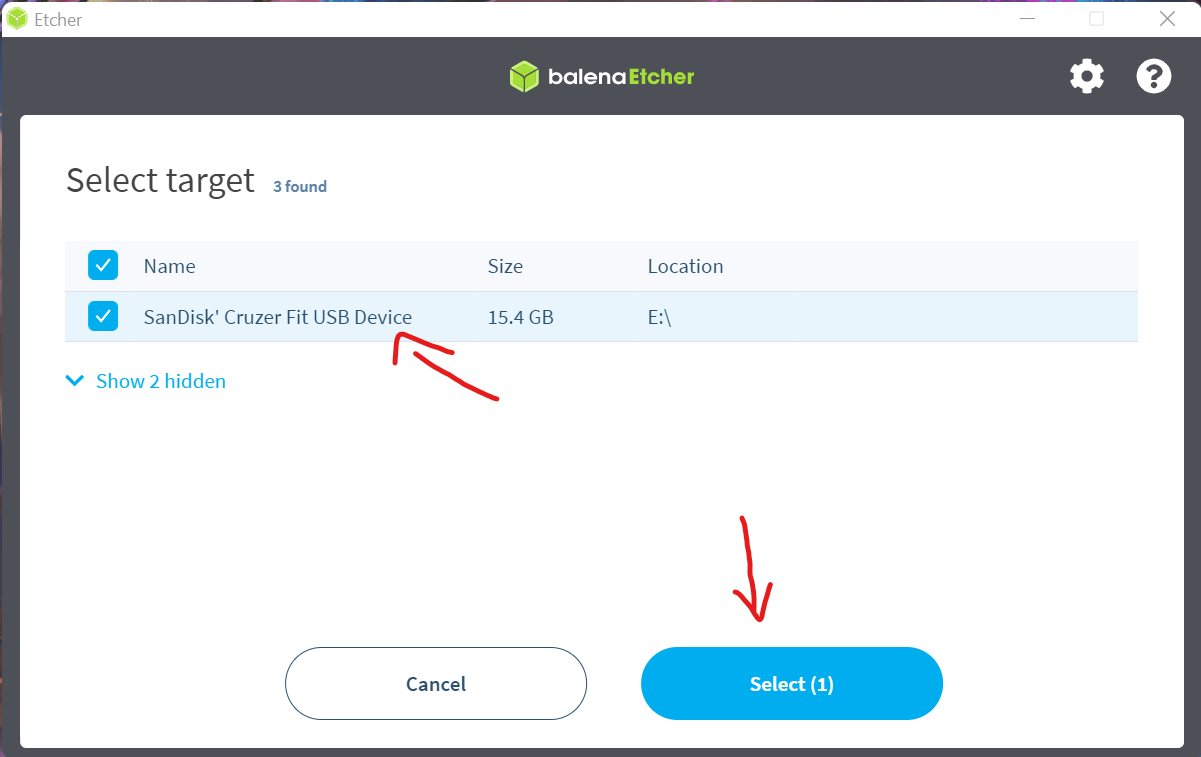
\includegraphics[width = 0.96\textwidth]{SelectUSBDevice2.png}
        \caption{Seleccionando el Drive}
        \label{fig:selectingDrive}
    \end{figure}
    \item Dele al botón de continuar (en balenaEtcher se llama Flash!)
    \begin{figure}[H]
        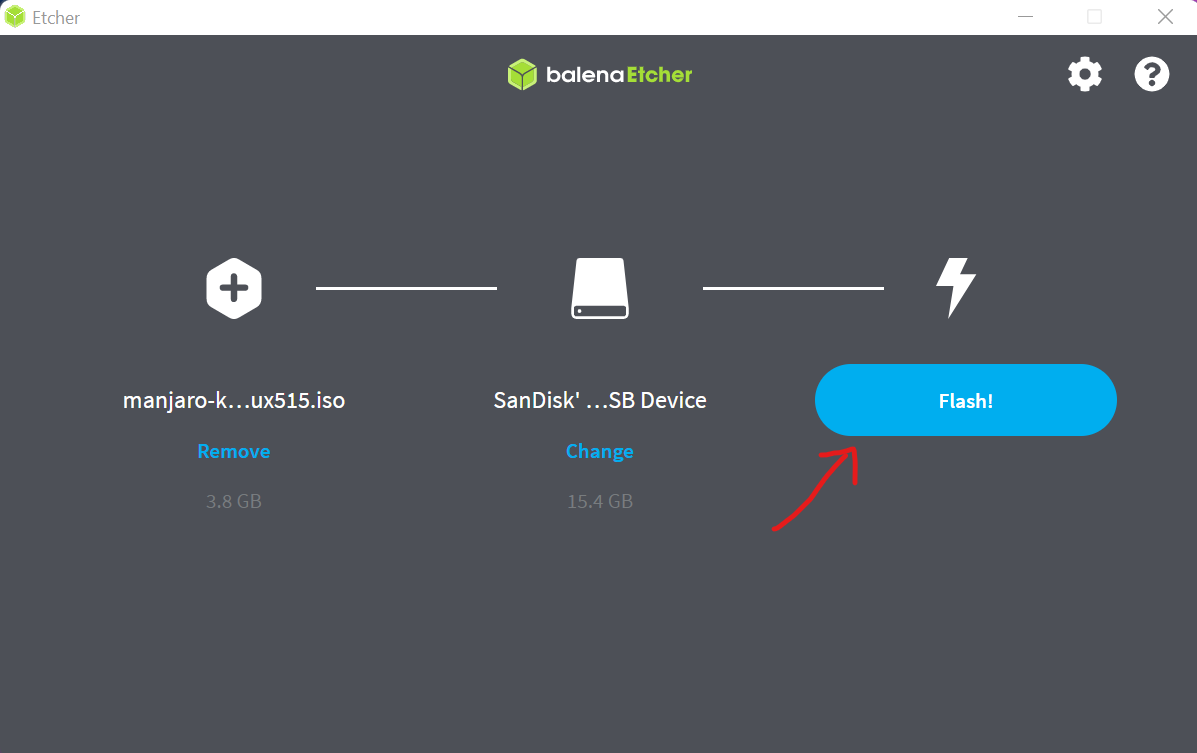
\includegraphics[width = 0.96\textwidth]{Flash!.png}
        \caption{Comenzando Flash!}
        \label{fig:flashing}
    \end{figure}
    \item Esperar, en esta parte Windows puede intentar de abrir el USB no lo va a lograr y va a preguntar si quiere formatear, puede cancelar esta operación balenaEtcher formatea automáticamente por uno.
    \begin{figure}[H]
        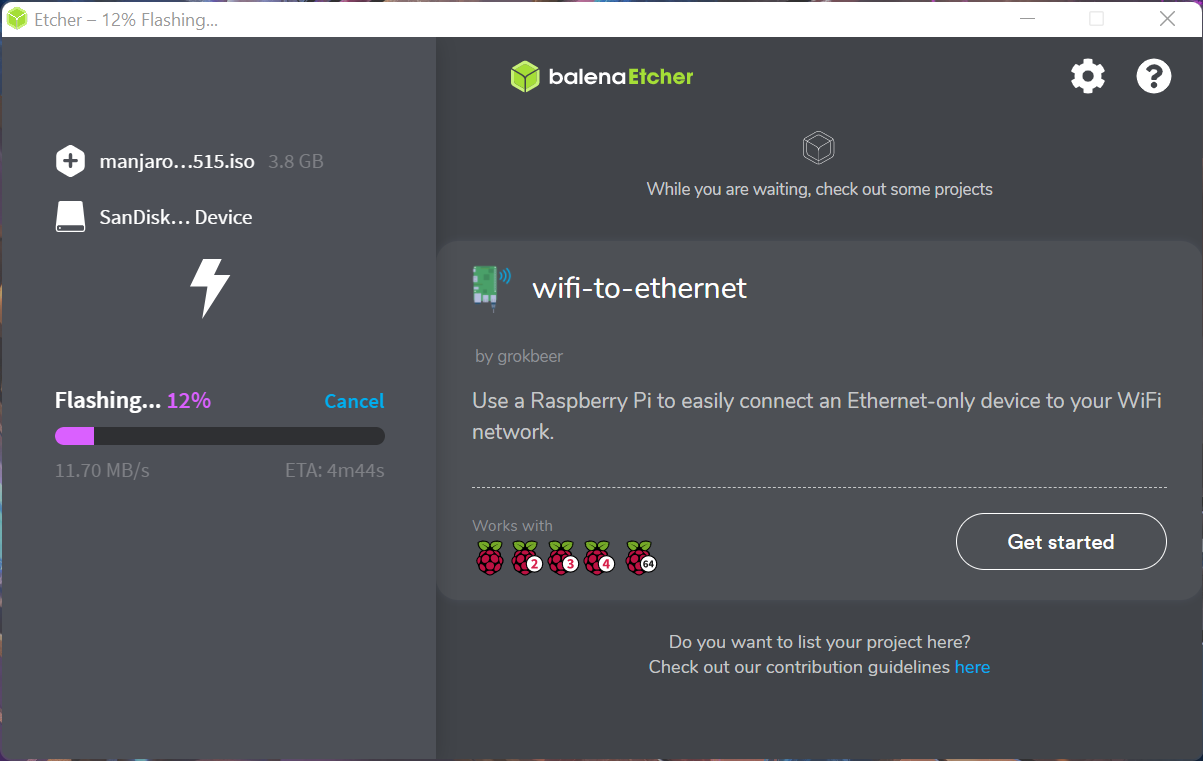
\includegraphics[width = 0.96\textwidth]{Waiting.png}
        \caption{Esperando}
        \label{fig:waiting}
    \end{figure}
    \item Repetir pasos 2-6
    \begin{figure}[H]
        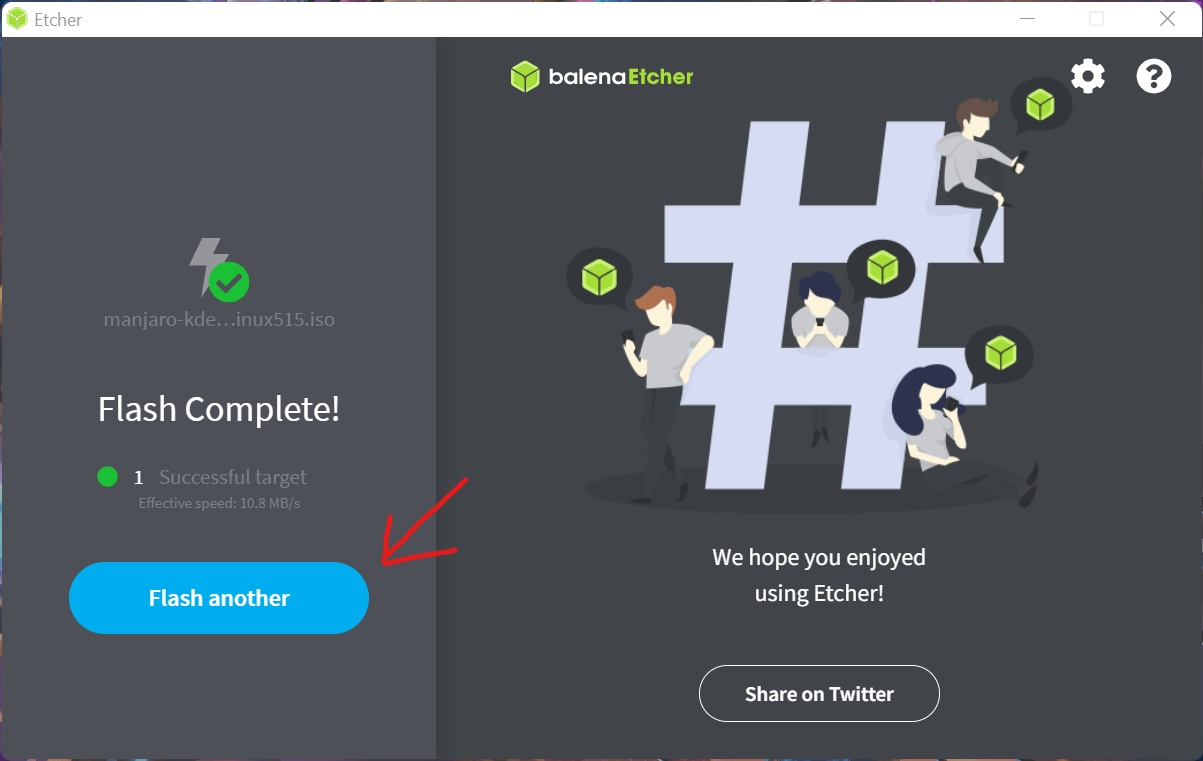
\includegraphics[width = 0.96\textwidth]{Repeat.png}
        \caption{Repetir}
        \label{fig:repeating}
    \end{figure}
\end{enumerate}

%------------------------------------------------------------------------------------
\section*{Investigación}
\phantomsection
\addcontentsline{toc}{section}{Investigación}

\begin{enumerate}
    \item ¿Qué es un USB booteable? \addcontentsline{toc}{subsection}{¿Qué es un USB booteable?}
    
    Según \cite{WhatIsABootableDrive}, un USB booteable es que un sistema de archivos esté en el USB y dejar que se pueda boot desde la computadora en vez de la llave malla como tal.

    \item ¿Qué otros programas (además de los mencionados aquí) se pueden utilizar para crear una USB booteable? \addcontentsline{toc}{subsection}{¿Qué otros programas (además de los mencionados aquí) se pueden utilizar para crear una USB booteable?}
    
    Softonic (\cite{SoftwareUSBFlashDrive}) creó una lista de software para hacer los USB booteables. Estos incluyen en orden:
    \begin{itemize}
        \item Rufus
        \item balenaEtcher
        \item Universal USB Installer
        \item USB AutoRun Creator
        \item muchos más
    \end{itemize}
    \item De la lista anterior, ¿Cuál programa le parece mejor? ¿Por qué? \addcontentsline{toc}{subsection}{De la lista anterior, ¿Cuál programa le parece mejor? ¿Por qué?}
    
    Por experiencia personal he usado Rufus y balenaEtcher:
    \begin{itemize}
        \item Rufus es bueno porque tiene varias opciones y manera de flashear, bootear o borrar el USB, pero para un principiante (por experiencia fue lo primero que usé), puede ser un poco abrumador.
        \item balenaEtcher es bueno porque toma como tres botones en una interfaz gráfica muy amigable para poder crear un USB booteable.
    \end{itemize}
    \item ¿Cuáles usos se le puede dar a una USB booteable? \addcontentsline{toc}{subsection}{¿Cuáles usos se le puede dar a una USB booteable?}
    \begin{itemize}
        \item Hacer la instalación de un servidor (\cite{CreateABootableDriveWindows})
        \item Tener una copia en caso de tener que recuperar una máquina (\cite{CreateABootableDriveWindows})
        \item Para poder instalar varias máquinas con las mismas configuraciones (como para un laboratorio de un centro educativo) (\cite{WhatIsABootableDrive})
        \item Instalar un sistema operativo nuevo (experiencia personal)
        \item Jugar con un sistema operativo nuevo sin modificar el existente (personalmente así es como se hizo en la final regional de la ICPC con donde se corría una instalación especial de Linux desde un USB booteable).
    \end{itemize}
    \item ¿Qué es un .ISO? \addcontentsline{toc}{subsection}{¿Qué es un .ISO?}
    
    Según \cite{WhatIsAnISO} un documento .ISO (del nombre de sistema de archivos de media óptico: ISO 9960), es una copia sector-por-sector del disco sin compresión.
    \item Indicar las características de los .ISO \addcontentsline{toc}{subsection}{Indicar las características de los .ISO}
    Según \cite{WhatIsAnISO} y \cite{FileExtension}, este archivo está basado en ISO-9660, es una copia exacta del disco original con estructura de directorio, información del sistema de archivos, atributos de archivos y códigos para bootear.
    

    \item ¿Cómo se puede conseguir un .ISO? \addcontentsline{toc}{subsection}{¿Cómo se puede conseguir un .ISO?}
    \begin{itemize}
        \item Descargar un archivo .ISO de un sistema operativo desde las páginas oficiales, como el ejemplo de antes con Manjaro.
        \item Según \cite{ISOConverters} hay varios softwares y maneras diferentes de convertir un folder a un archivo .ISO, que como se comentó antes es una copia exacta.
    \end{itemize}

\end{enumerate}

%----------------------------------------------------------------------------------------------------------------------------------------------------------------------
\section*{Conclusión}
\phantomsection
\addcontentsline{toc}{section}{Conclusión}

En este laboratorio se explora como hacer un USB booteable, al igual que datos de este y el archivo .ISO que se usa para crearlo.Se evalua las diferentes maneras en las que se puede usar un USB booteable.

\newpage
% Referencias
\renewcommand\refname{\large\textbf{Referencias}}
\bibliography{ref}

\end{document}